
\chapter[Related Works]{State of the art}
\graphicspath{ {images/stateOfArt} }



\section{Software visualization}


\begin{wrapfigure}{r}{0.3\textwidth}

  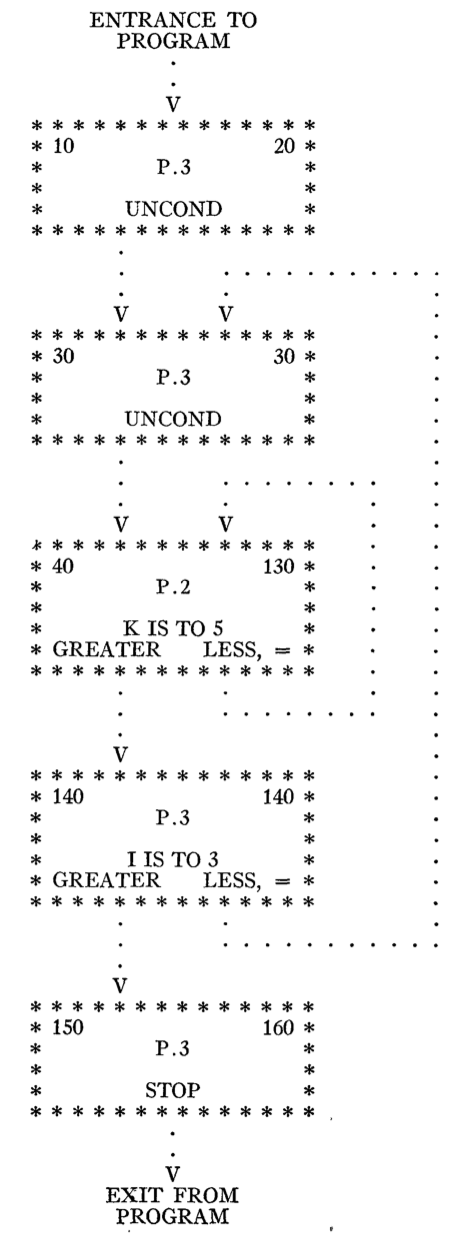
\includegraphics[width=0.9\linewidth]{Haibt1959_Flowchart.png} 
  \caption{Flowchart presented by Haibt in 1959}
  \label{fig:Haibt1959_Flowchart}

\end{wrapfigure}

Software maintenance and evolution are essential parts of the software development lifecycle. Both require that developers deeply understand their system. 
Mayrhauser and Vans defined {\it program comprehension} as a process that "{\it knowledge to acquire new knowledge}" \cite{VonMayrhauser1995}. 
Generally, programmers possess two types of knowledge: general knowledge and software-specific knowledge. 
Software comprehension aims to increase this specific knowledge of the system, and, it can leverage some software visualization techniques for this purpose. 
Software visualization supports the understanding a software systems
by visually presenting various information about it, e.g., its architecture, source code, or behavior.
Stasko et al.\cite{Stasko2008} conducted a study in 1998 that shows how visualization arguments human memory since it works as external cognitive aid and thus, improves thinking and analysis capabilities. \\

% \subsection*{History of software visualization}



The earliest software visualization techniques in the literature used 2D diagrams. 
For example, Haibt, the first to use them in 1959, provided a graphical outline of a program and its behavior with flowcharts \cite{Haibt1959}. 
As shown in Figure \ref{fig:Haibt1959_Flowchart}, they were 2D diagrams that described the execution of a program.
 He wrapped each statement in a box, representing the control flow with arrows.
Ten years later, Knuth also confirmed the effectiveness of flowcharts \cite{Knuth1963}. 

Unfortunately, around that time, programs were affected by a lack of readability.
Therefore, it introduced a tool to generate visualizations from the software documentation automatically. 
Nassi and Schneiderman\cite{Nassi1973}, in 1973, introduced the Nassi–Shneiderman diagram (NSD), able to represent the structure of a program. 
The diagram was divided into multiple sub-block, each with a given semantic based on its shape and position. 


The 80s registered two main directions of software visualization. The first was the source code presentation.
For example, Hueras and Ledgard \cite{Hueras1977} then Waters \cite{Waters1983} developed techniques to format the source code with a prettyprinter. 
The second direction was the program behavior, used mainly for educational purposes. One of that period's most prominent visualization systems was Balsa-II \cite{Brown1988}.

Balsa-II was a visualization system that, through animations, displayed the execution of an algorithm.
Programmers were able to customize the view and the control execution of the algorithm, to understand them with a modest amount of effort. 
The program was domain-independent, and users could use it with any algorithm. 



Around the end of the 80s, Müller et al. \cite{Mueller1988} released Rigi, a tool used to visualize large programs.
It exploited the graph model, augmented with abstraction mechanisms, to represent systems components and relationships. 

\begin{figure}[H]
  \minipage{0.33\textwidth}
    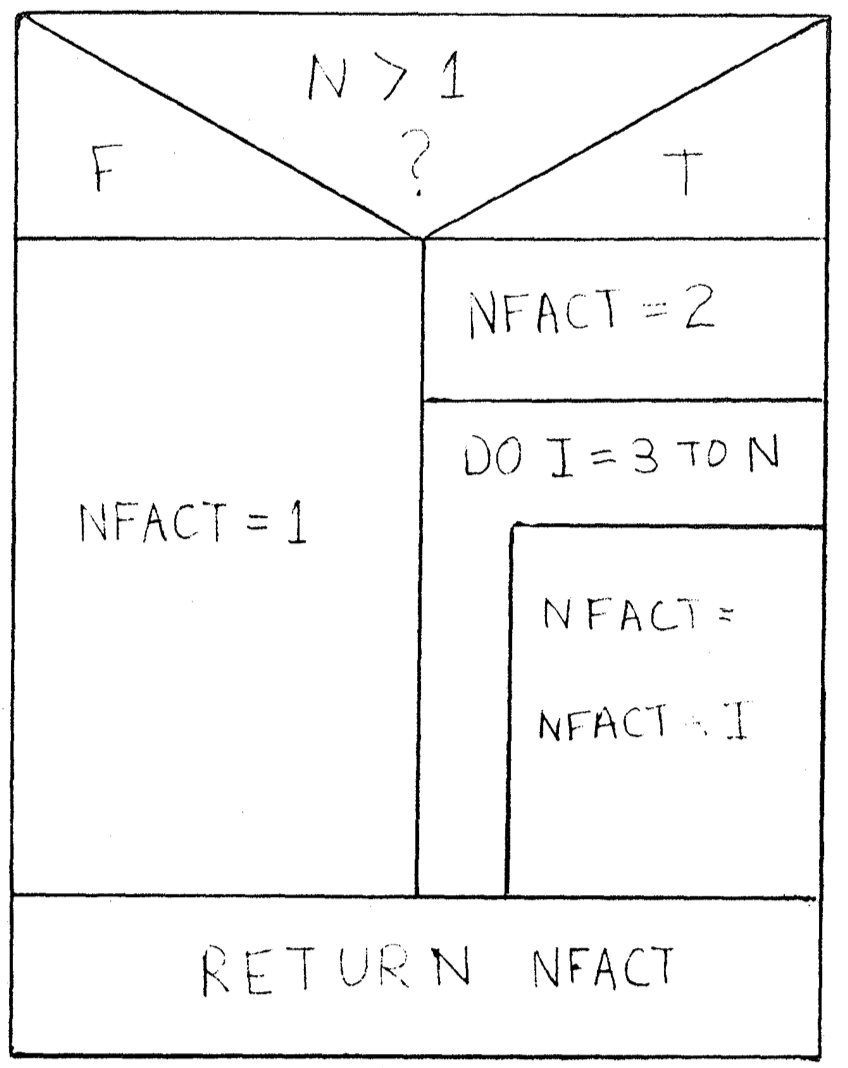
\includegraphics[width=0.8\linewidth]{Nassi1973_NSD.png}
    \label{fig:Nassi1973_NSD}
    \caption{NSD of the factorial function.}
  \endminipage\hfill
  \minipage{0.33\textwidth}
    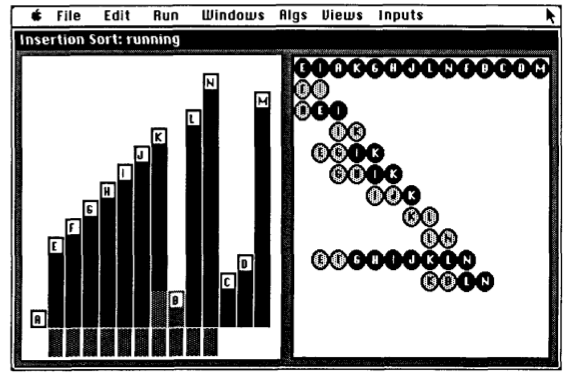
\includegraphics[width=\linewidth]{Brown1988_BalsaII.png}
    \caption{Balsa-II}
  \endminipage\hfill
  \minipage{0.33\textwidth}
  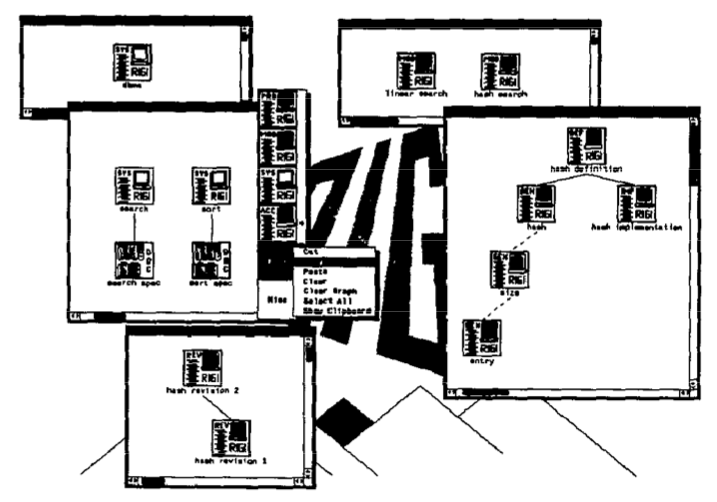
\includegraphics[width=\linewidth]{Mueller1988_Rigi.png}
  \caption{Rigi}
\endminipage\hfill
  \end{figure}


  % The growing number of object-oriented programming languages emerging in the mainstream raised 
  % the interest in understanding not only the structure, but also the behavior of systems written according to this paradigm. 
  % Kleyn et al. proposed GraphTrace [KG88], a tool using concurrently animated views to visualize dynamic information,
  % Myers's taxonomy of program visualization systems
  % Price et al. proposed a more detailed taxonomy


The 1990s recorded more interest in the field of software visualization. 
In 1992, Erik et al. introduced a new technique to visualize line-oriented statistics \cite{Eick1992}. 
It was embodied in Seesoft, a software visualization system to analyze and visualize up to 50,000 lines of code simultaneously. 
On their visualization, each line was mapped to a thin row. Each row was associated with a color that described a statistic of interest.
One year later, De Pauw et al. \cite{DePauw1993} introduced Jinsight, a tool able to provide animated views of object-oriented systems's behavior. 

\begin{figure}[H]
  \minipage{0.5\textwidth}
    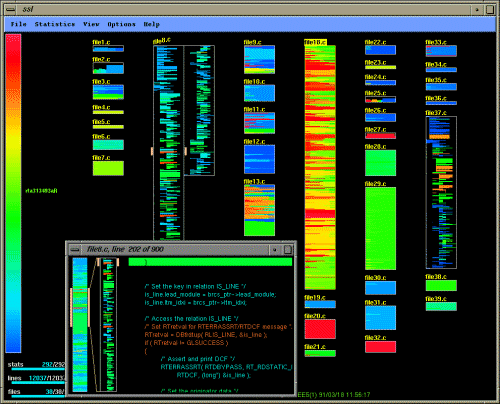
\includegraphics[width=0.8\linewidth]{Eick1992_Seesoft.png}
    \caption{Seesoft}
  \endminipage\hfill
  \minipage{0.5\textwidth}
    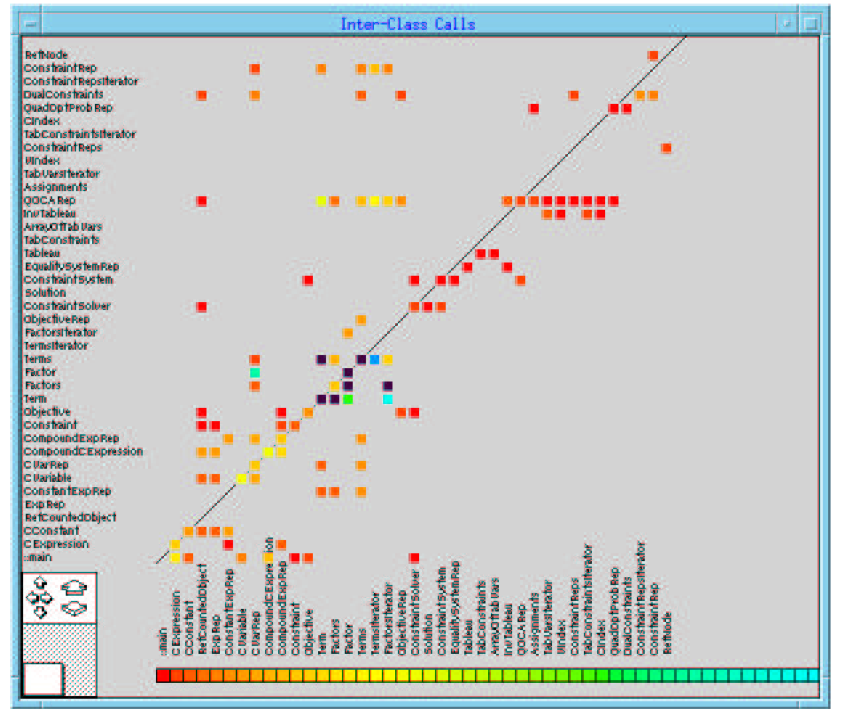
\includegraphics[width=0.8\linewidth]{DePauw1993_Jinsight.png}
    \caption{Jinsight}
  \endminipage\hfill
\end{figure}

% he first contributors to software evolution visualization were Holt and Pak in 1996, who used their tool called GASE [HP96]
% 		GASE: visualizing software evolution-in-the-large 

That period was favorable also for experimenting with novel research directions for visualization, 
such as 3D visualization and Virtual Reality. 

% In 1995, Reiss presented a configurable engine for building 3D visualization of programs called PLUM
In 1998, Chuah and Erick \cite{Chuah1998} proposed three different techniques to visualize project data. 
They exploited the concept of glyphs, a graphical object that represents data through visual parameters. 
The first technique was the Timewhell glyph, used to visualize time-oriented information (number of lines of code, number of errors, number of added lines). 
The second technique was the 3D wheel glyph; it encoded the same attributes of the time wheel, and additionally, it used the height to encode time. 
Infobug glyph was the last technique, where each glyph was composed of four parts, each representing essential data of the system, such as time, code size and the number of added, deleted, or modified code lines. \newline

\begin{figure}[H]
\minipage{0.32\textwidth}
  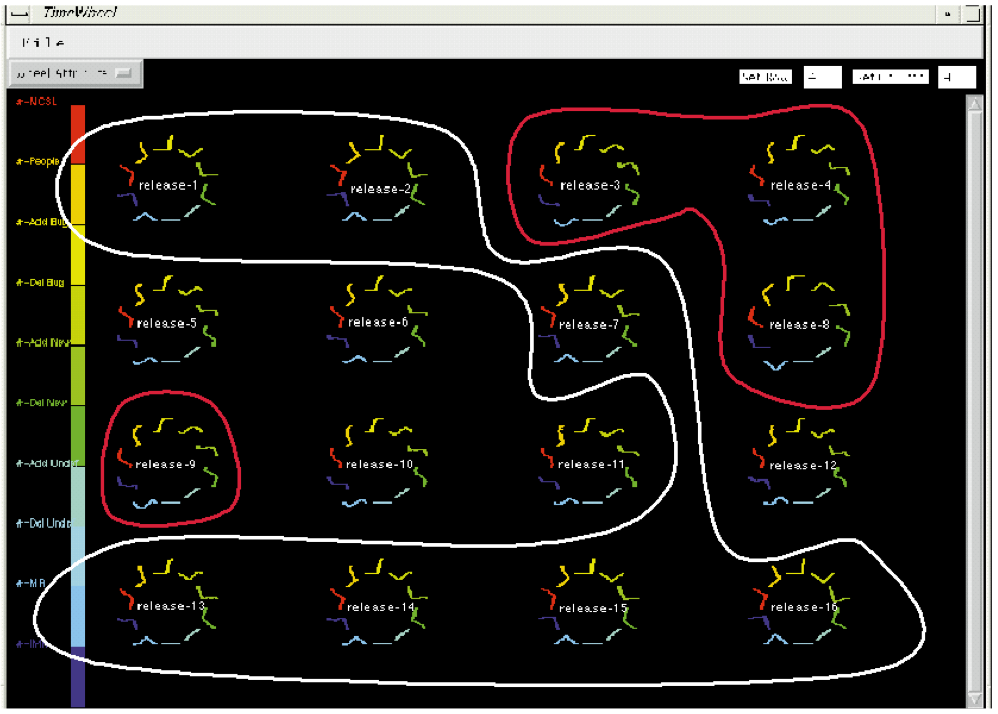
\includegraphics[width=\linewidth]{Chuan1.png}
  \caption{Timewhell}
\endminipage\hfill
\minipage{0.32\textwidth}
  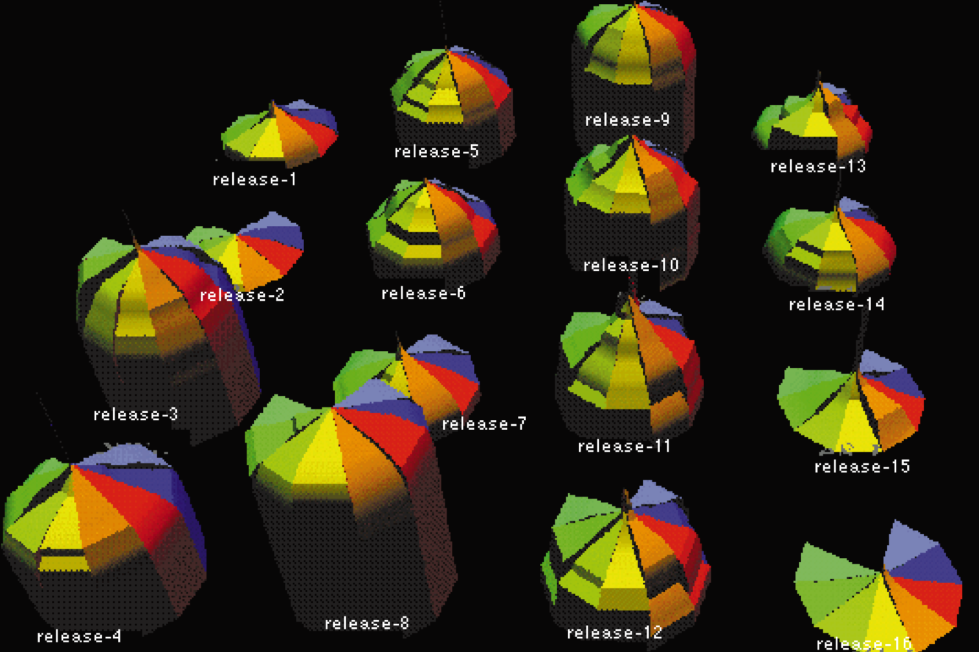
\includegraphics[width=\linewidth]{Chuan2.png}
  \caption{3D wheel}
\endminipage\hfill
\minipage{0.32\textwidth}%
  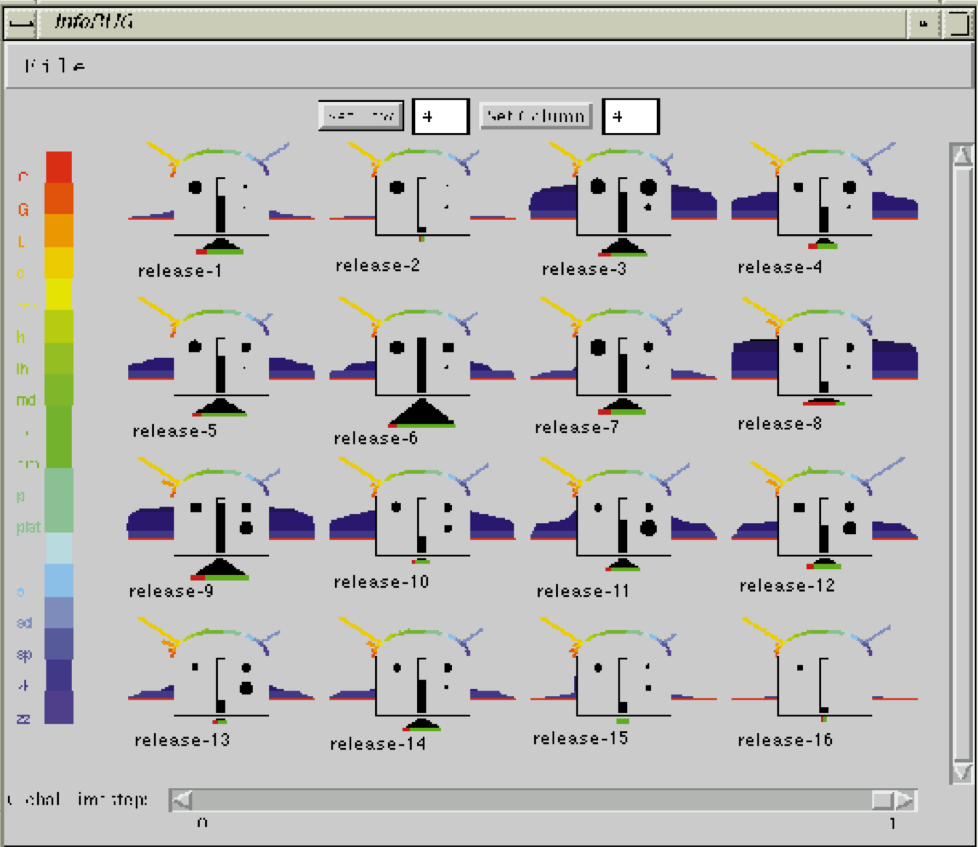
\includegraphics[width=\linewidth]{Chuan3.png}
  \caption{Infobug}
\endminipage
\end{figure}

Also in 1998, Young and Munro \cite{Young1998} explored representations of software for program comprehension in VR. 
Finally, in 1999, Jacobson et al. \cite{Jacobson1999} introduced what we now know as de facto the standard language to visualize the design of a system: UML. 


% Edward Tufte has influenced the entire field of information visualization, including software visualization.
% 	[Tuf90] Edward Tufte. Envisioning Information. Graphics Press, 1990.
% 	[Tuf97] Edward Tufte. Visual Explanations. Graphics Press, 1997.
% 	[Tuf01] Edward Tufte. The Visual Display of Quantitative Information. Graphics Press, 2nd edition, 2001.

% \subsection{Software evolution visualization}
%https://www.inf.usi.ch/faculty/lanza/Downloads/Gall2006a.pdf
Before the beginning of the 21st century, thanks to the spread of version control systems and the open-source movement, 
visualizing the evolution of a system became a more feasible activity since there was more publicly accessible system information.   
As a result, many researchers focused their work on software evolution visualization.

Lanza \cite{Lanza2001} introduced the concept of the Evolution Matrix. 
It was a way to visualize the evolution of software without dealing with a large amount of complex data. 
Furthermore, this approach was agnostic to any particular programming language. 
The Evolution Matrix aimed to display the evolution of classes in object-oriented software systems. 
Each column represented a version of the software; each row represented a different version of the same class.
Cells were filled with boxes whose size depended on evolutionary measurements. 
The shape of the matrix could also be used to infer various evolutionary patterns.

\begin{figure}[H]
\minipage{0.49\textwidth}
  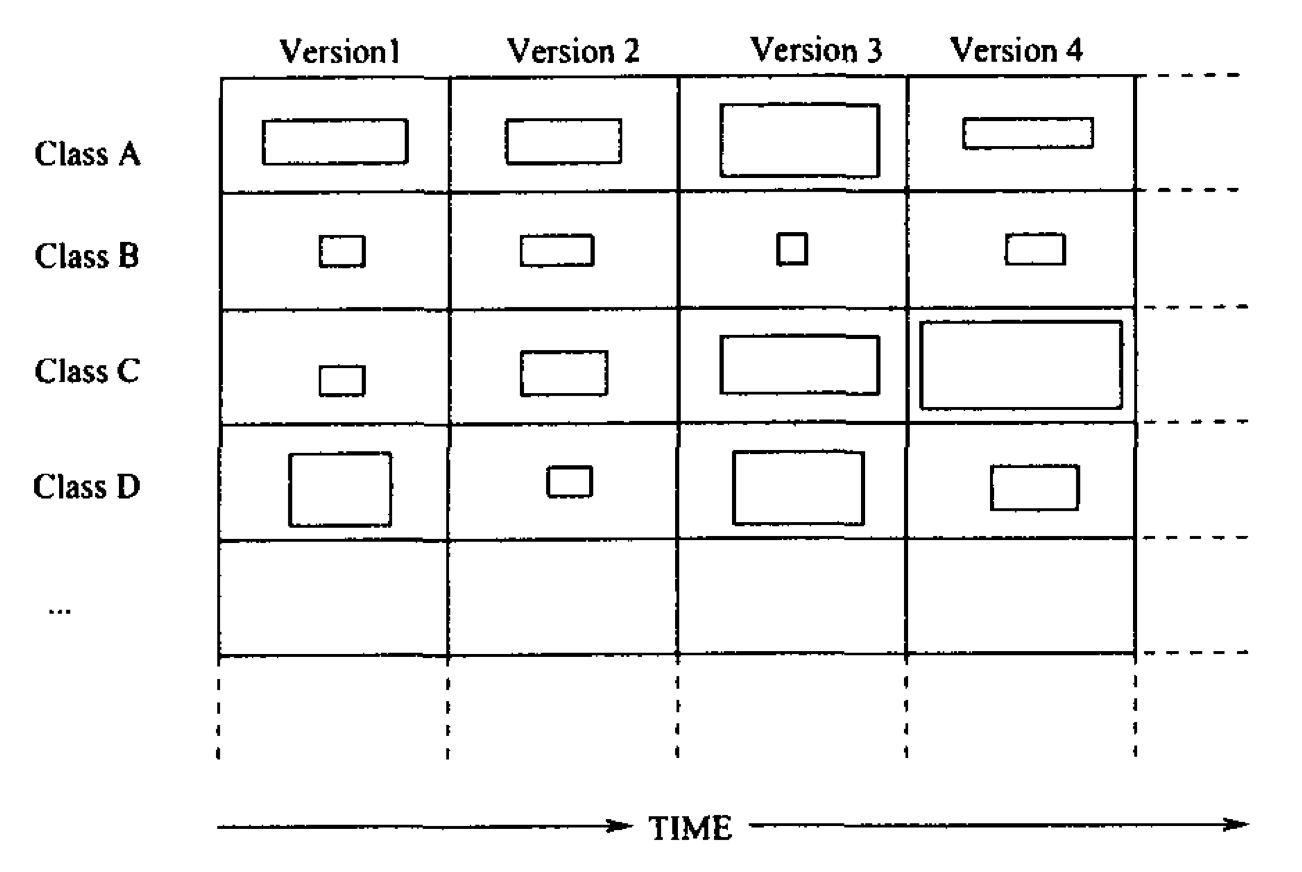
\includegraphics[width=\linewidth]{EvolutionMatrix1.png}
  \caption{A schematic display of the Evolution Matrix}
\endminipage\hfill
\minipage{0.49\textwidth}
  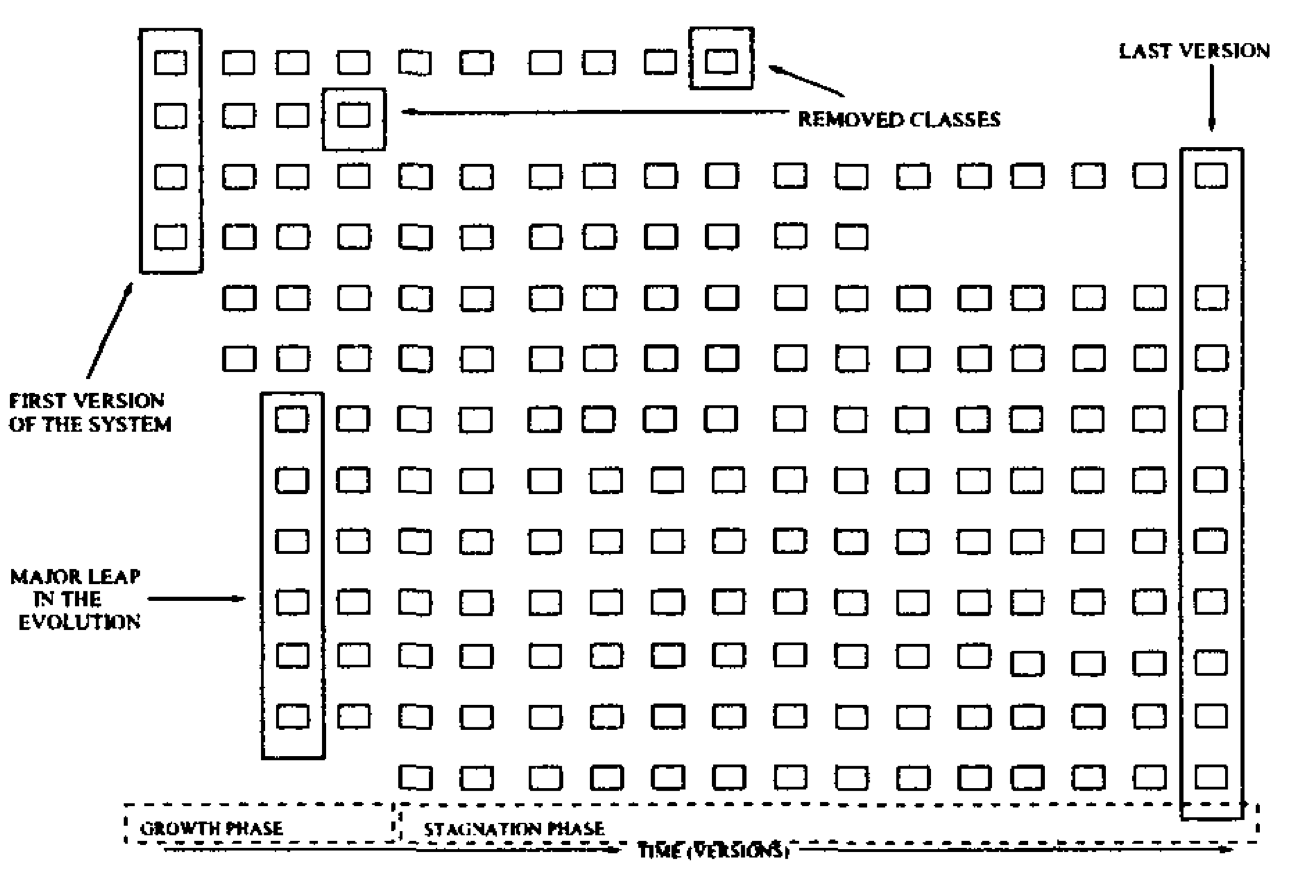
\includegraphics[width=\linewidth]{EvolutionMatrix2.png}
  \caption{Some characteristics of the Evolution Matrix}
\endminipage\hfill
\end{figure}


Taylor and Munro \cite{Taylor2002},  demonstrated that it was possible to use the data contained in a version control repository to visualize the evolution of a system.
They developed Revision Tower, a tool that showed change information at the file level. 
Pinzger et al. \cite{Pinzger2005} visualized the evolution of a software system through Kivat diagrams.
RelVis, their tool, was able to depicted a multivariate visualization of the evolution of a system.
During the same year, Ratzinger et al. presented EvoLens \cite{Ratzinger2005}, a visualization approach and tool to 
explore evolutionary data through structural and temporal views.  
During the same year, Langelier et al. \cite{Langelier2005} investigated the interpretation of a city metaphor 
\cite{Knight2000} to add a new level of knowledge to the visual analysis.

D’Ambros and Lanza \cite{DAmbros2006} introduced the concept of Discrete Time Figure concept. It was a 
 visualization technique that embedded both historical and structural data in a simple figure. 
Their approach depicted relationships between the histories of a system and bugs. 
They also presented the Evolution Radar \cite{DAmbros2006a}, a novel approach to visualize module-level and file-level logical coupling information.

\begin{figure}[H]
  \minipage{0.33\textwidth}
    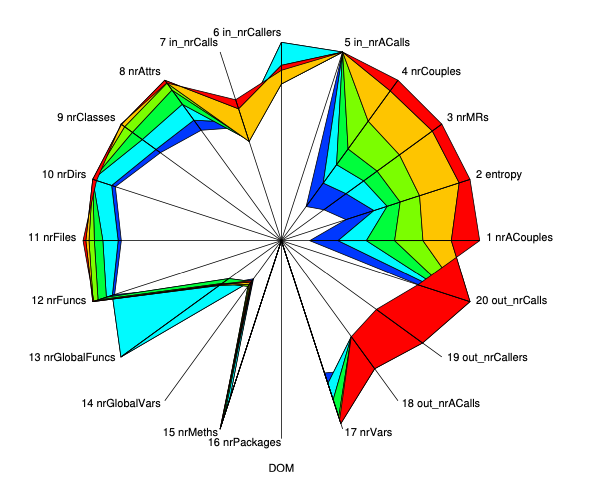
\includegraphics[width=\linewidth]{Pinzger2005_RelVis.png}
    \caption{RelVis}
  \endminipage\hfill
  \minipage{0.33\textwidth}
    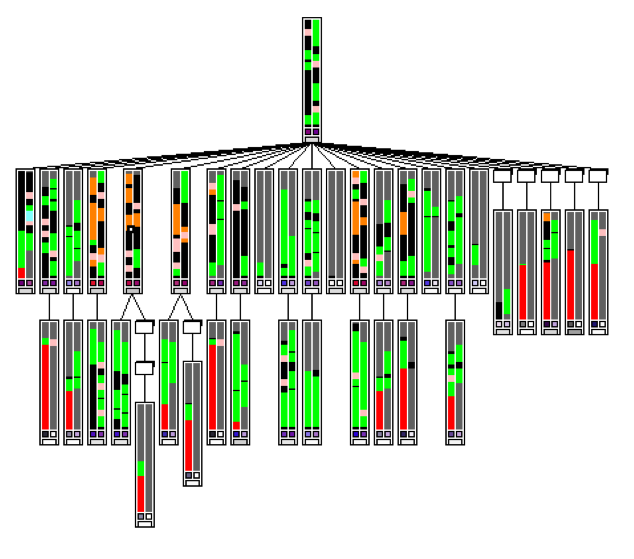
\includegraphics[width=\linewidth]{DAmbros2006.png}
    \caption{Tree of Discrete Time Figures}
  \endminipage\hfill
  \minipage{0.33\textwidth}
  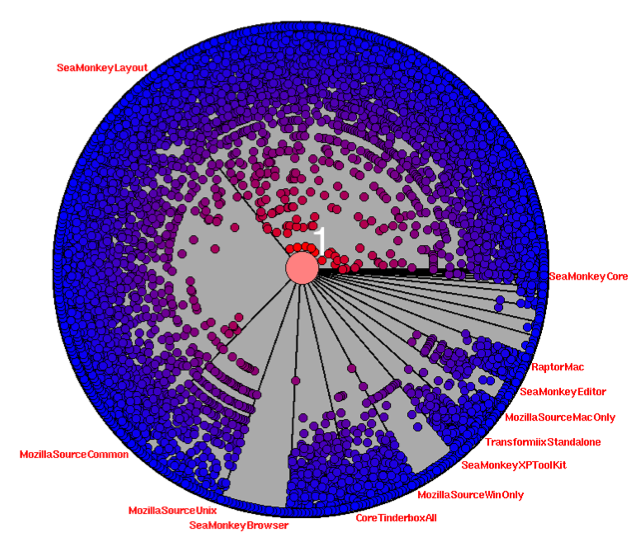
\includegraphics[width=\linewidth]{DAmbros2006a_EvoRadar.png}
  \caption{Evolution Radar}
\endminipage\hfill
  \end{figure}
  

Steinbrückner and Lewerentz \cite{Steinbrueckner2010} described a three-staged visualization approach to visualize large software systems. 
Thir visualization was supported by a tool called Evo-Streets. 
Each stage of their approach was responsible for representing a different aspect of the system with the city metaphor. 


\begin{figure}[H]
  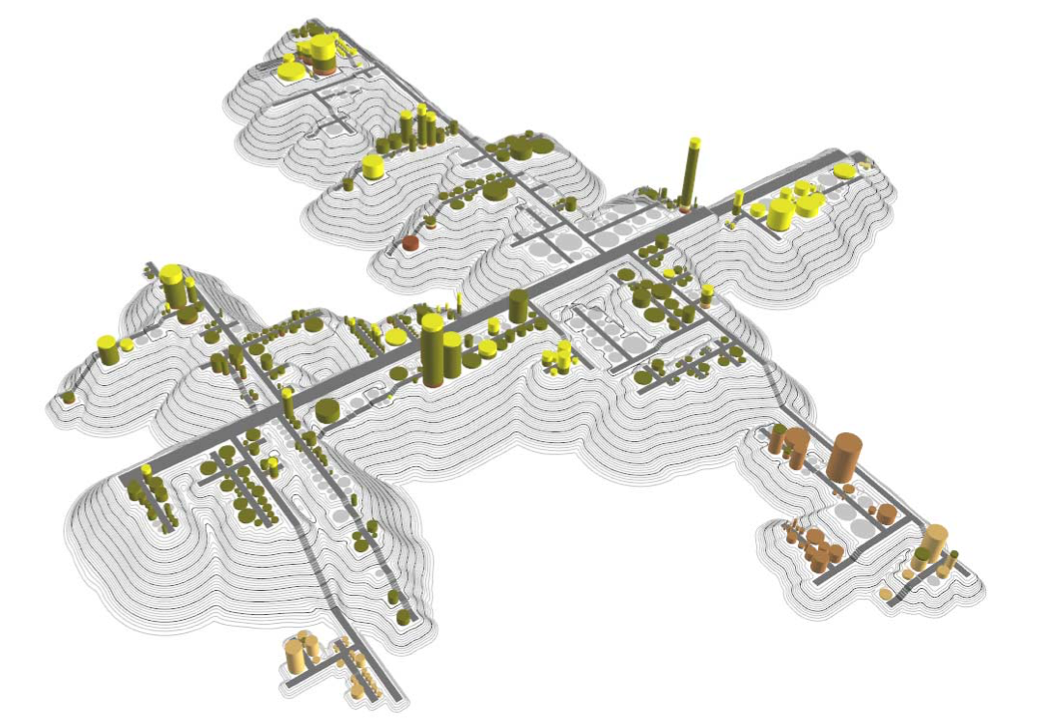
\includegraphics[width=0.9\linewidth]{Steinbrueckner2010.png} 
  \caption{Evo-Streets}
\end{figure}

Wettel revised the city metaphor to represent metrics meaningfully  \cite{Wettel2011}. 
In his thesis, he represented packages as districts and classes as buildings.
The metaphor was used for various purposes, e.g., reverse engineering, program comprehension, software evolution or software quality analysis. 
He claimed that the city metaphor brought visual and layout limitations; for example, not all visualization techniques fit well.
Under those circumstances, he preferred simplicity over accuracy,
so he obtained a simple visual language that facilitated data comprehension. His approach was implemented as software visualization tool 
called CodeCity. 


\begin{figure}[H]
  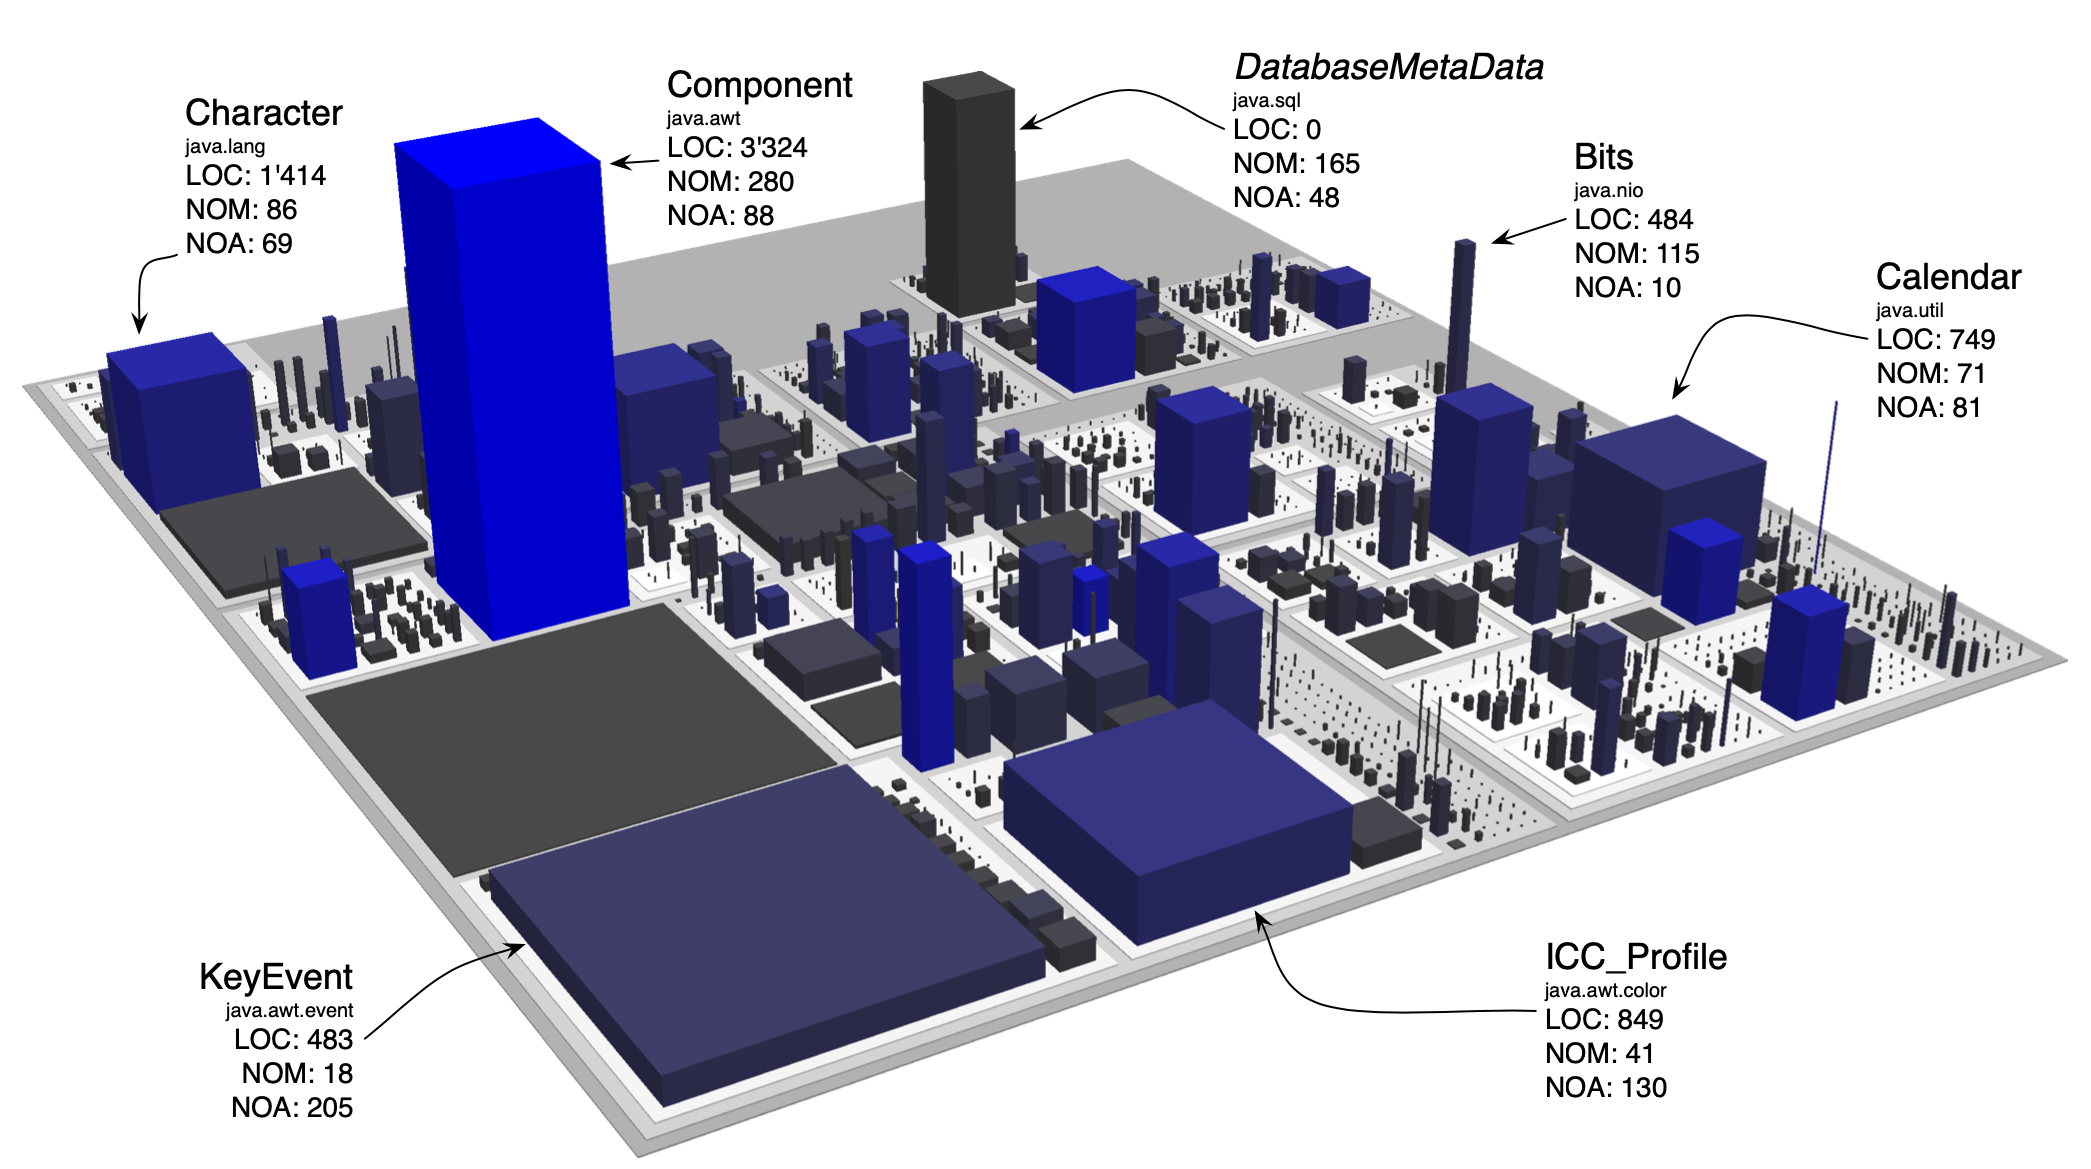
\includegraphics[width=0.9\linewidth]{CodeCity.png} 
  \caption{CodeCity}
\end{figure}



% ChronoTwigger 2014 https://ieeexplore.ieee.org/abstract/document/6980223
Ens et al. \cite{Ens2014} applied visual analytics methods to software repositories.
His approach helped users comprehend co-evolution information by visualizing how source and test files were developed together. 

% NN 2015 https://ieeexplore.ieee.org/document/7329727
Kapec et al. \cite{Kapec2015} proposed a graph analysis approach with augmented reality. 
They made a prototype of a tool that provided a graph-based visualization of software, and then they studied some interaction methods to control it with augmented reality.

% CuboidMatrix 2016 https://ieeexplore.ieee.org/document/7780168
Schneider et al. \cite{Schneider2016} presented a tool, CuboidMatrix, that employed a space-time cube metaphor to visualize a software system. 
A space-time cube is a well-known 3D representation of an evolving dynamic graph. 

% CityVR 2017 https://ieeexplore.ieee.org/abstract/document/8094470
Merino et al. \cite{Merino2017} aimed to augment software visualization with gamification. 
They introduced CityVR, a tool that displays a software system through the city metaphor with a 3D environment. 
Working with virtual reality, they scaled the city visualization to the physically available space in the room. 
Therefore, developers needed to walk to navigate the system. 

\begin{figure}[H]
  \minipage{0.32\textwidth}
    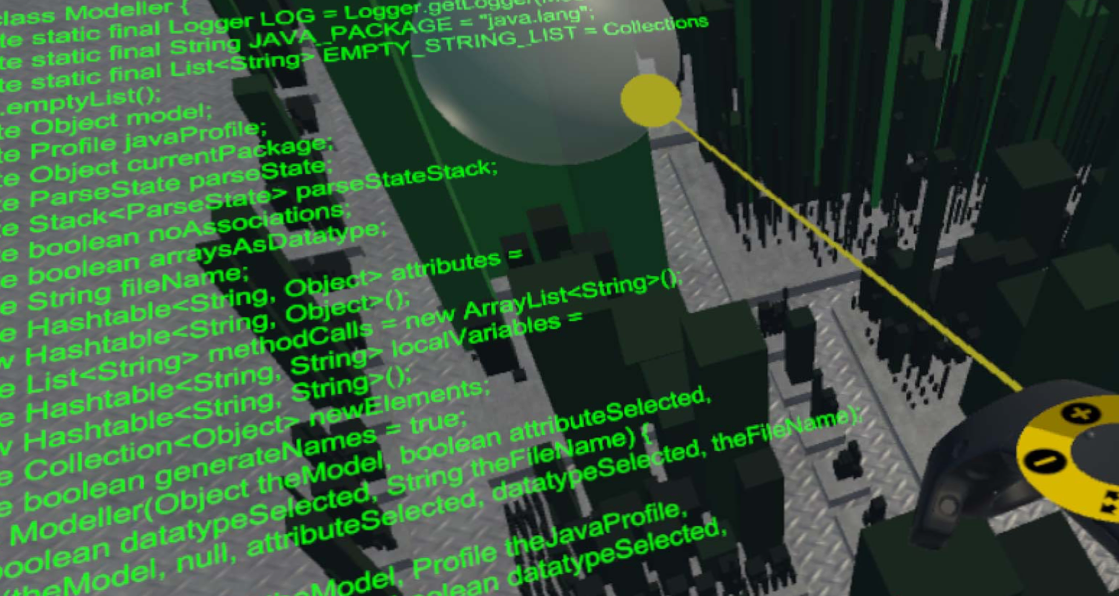
\includegraphics[width=\linewidth]{CityVR.png}
    \caption{CityVR}
  \endminipage\hfill
  \minipage{0.32\textwidth}
    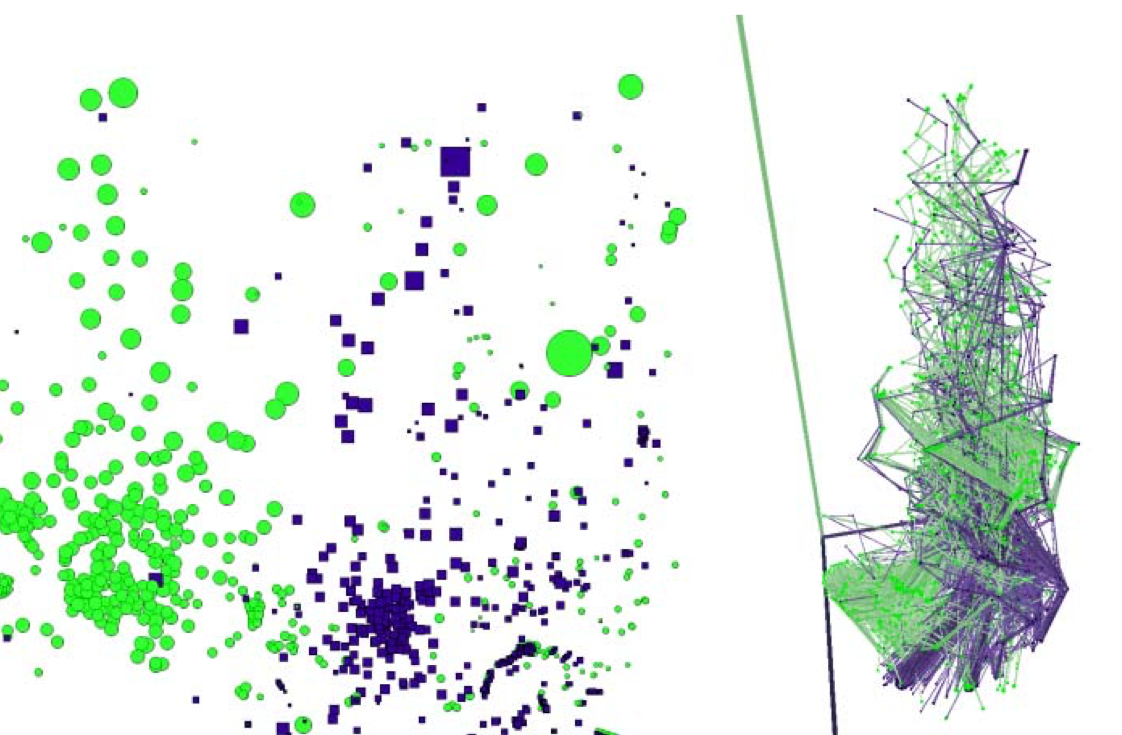
\includegraphics[width=\linewidth]{ChronoTwigger.png}
    \caption{ChronoTwigger}
  \endminipage\hfill
  \minipage{0.32\textwidth}%
    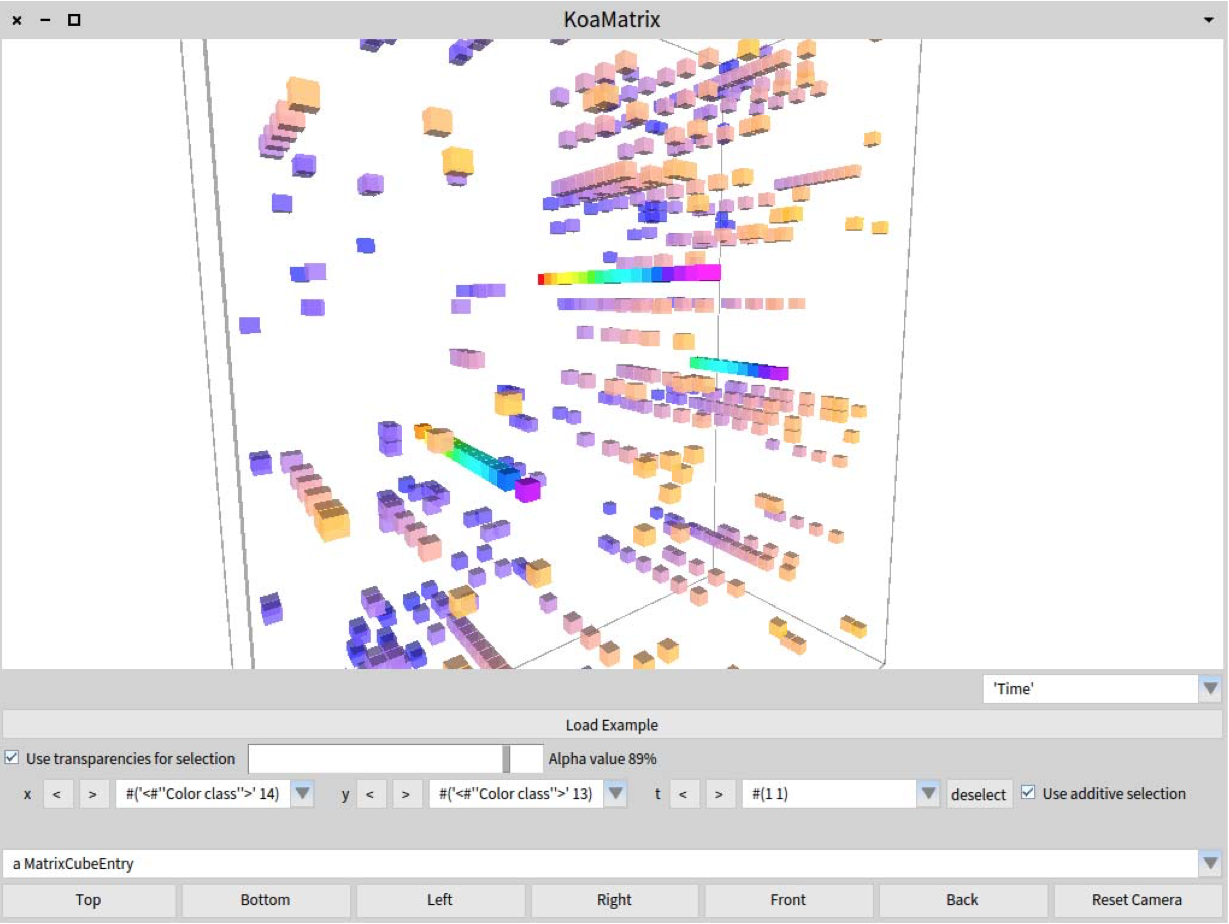
\includegraphics[width=\linewidth]{CuboidMatrix.png}
    \caption{CuboidMatrix}
  \endminipage
  \end{figure}
  


% Code Park 2017 https://ieeexplore.ieee.org/abstract/document/8091185
Khaloo et al. \cite{Khaloo2017} revised the idea of gamification with a 3D park-like environment.
 They mapped each class in the codebase with a facility. The wall structure depended on constituent parts of the class e.g., methods and signatues. 

% Evo-Clocks 2019 https://ieeexplore.ieee.org/document/8900965
Finally, we mention Alexandru et al., who proposed a method to visualize software structure and evolution, 
with reduced accuracy and a fine-grained highlighting of changes in individual components \cite{Alexandru2019}. 

\begin{figure}[H]
  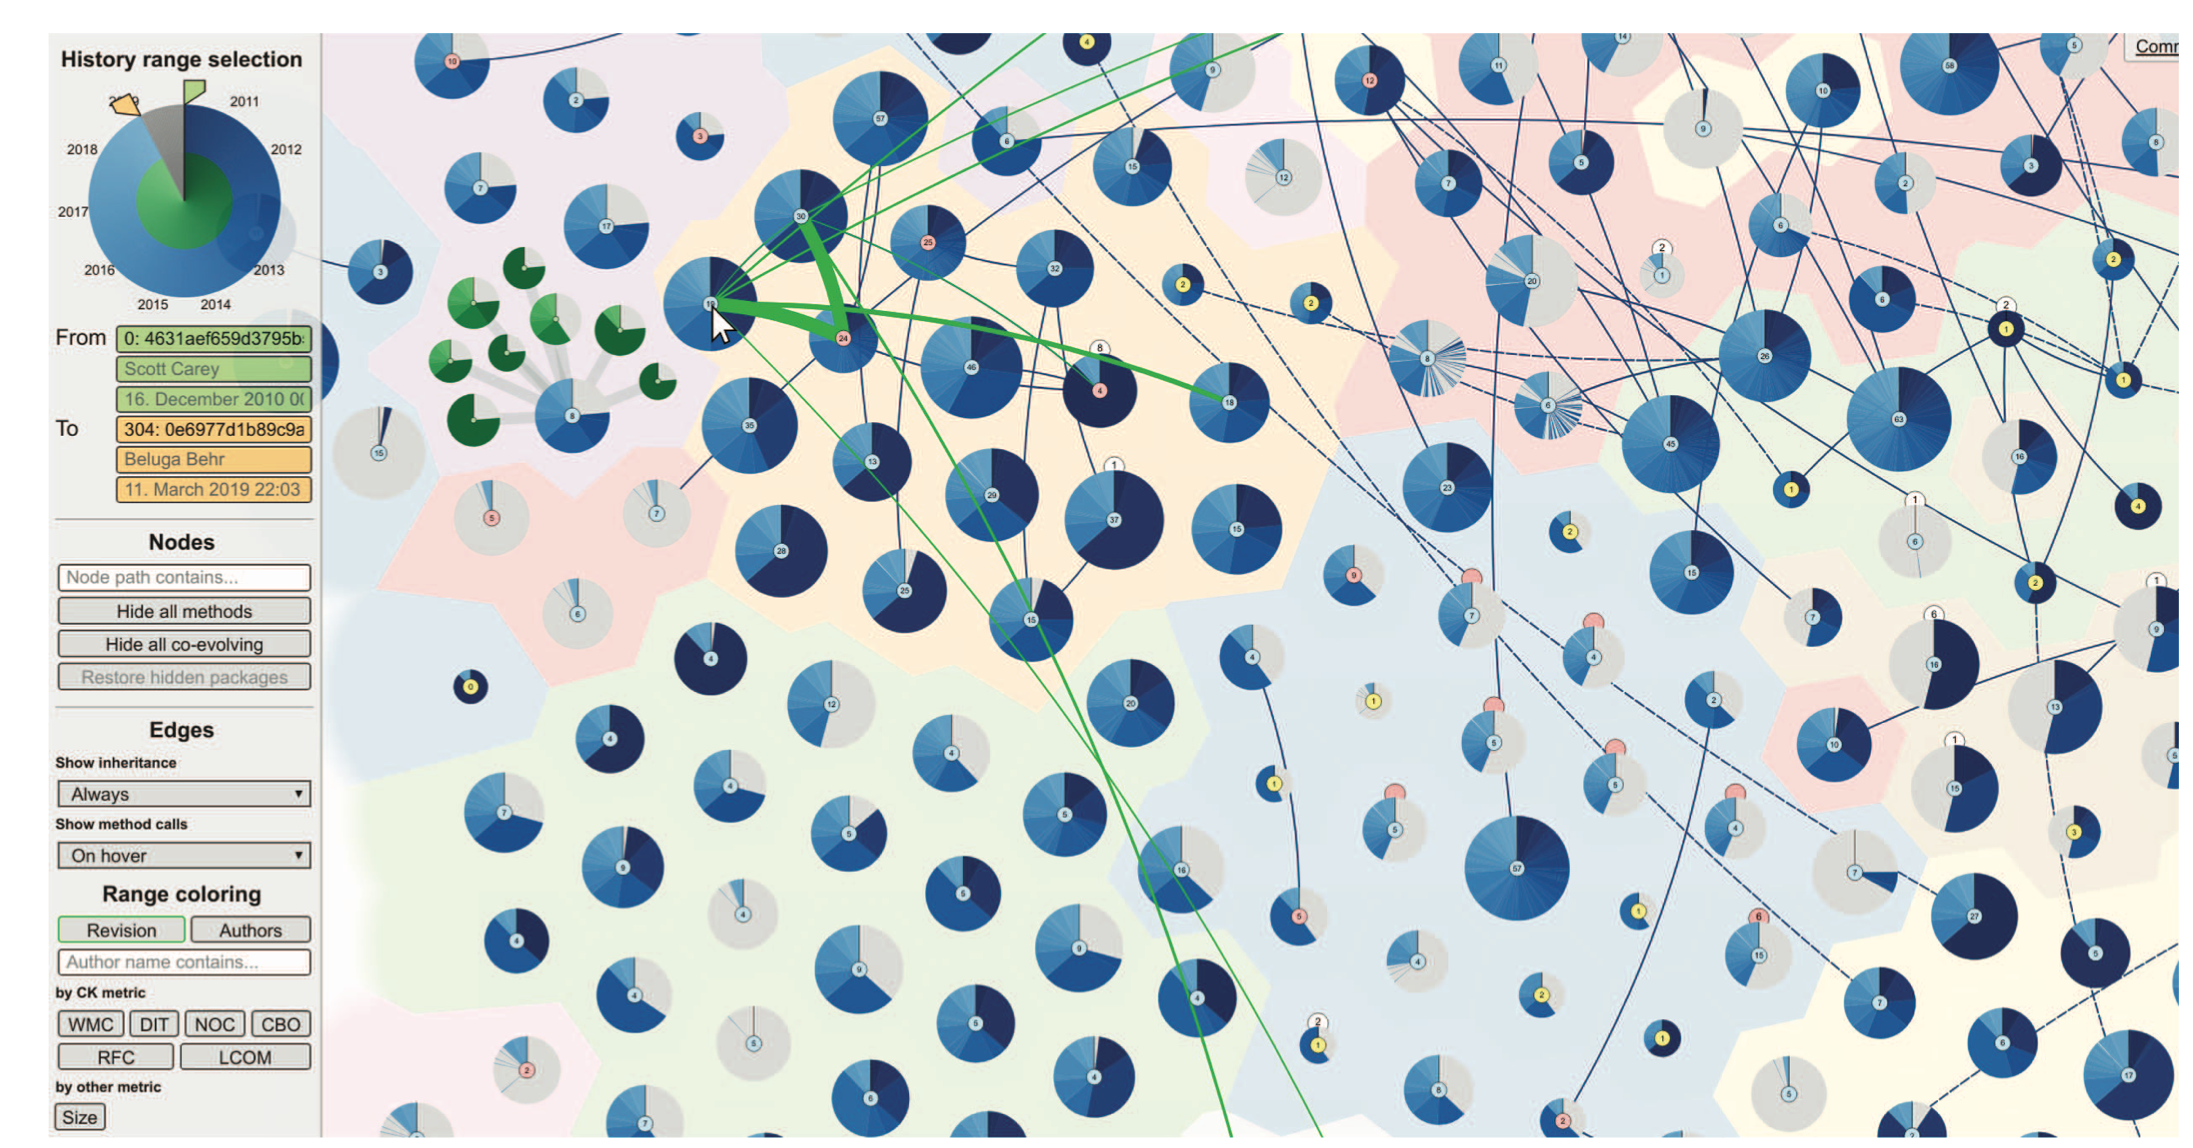
\includegraphics[width=0.9\linewidth]{Alexandru_EvoClock.png} 
  \caption{Evo-Clock}
\end{figure}


\section{Mining software repositories}

Software repositories contain historical data about the evolution of a software system. 
Thanks to the spread of the git protocol, and consequently of GitHub, the largest code hosting website, 
Mining software repositories (MSR) became a popular research field. 

% The promises and perils of mining GitHub  https://dl.acm.org/doi/abs/10.1145/2597073.2597074
In 2022, the number of GitHub repositories lays around 200 million.
Even if it seems a promising source of data, Kalliamvakou et al. \cite{Kalliamvakou2014} raised some issues with its mining.
They evidenced that a repository doens't always match with a project. 
A reason of this can be found in the fact that most repositories had had very few commits before becoming inactive.
When they made their research, over the 70 percent of the GitHub projects were personal, and some of them weren't used for software development. 
Finally, the last perils that they raise, were related to GitHub features that are not properly used by software developers.
To find actively developed repositories, they considered only projects with a good balance between number of commits, 
number of pull requests and number of contributors. 


% PyDriller https://dl.acm.org/doi/abs/10.1145/3236024.3264598
Spadini et al. \cite{Spadini2018} developed a Python framework, called PyDriller, that enables users to mine software repositories. 
They showed that their tool can be used to extract information about the evolution of a software system from any git repository.  

\newpage

\section{Data sonification}

External auditory representations of programs (known as program auralisation) is a researching field that 
is getting even more interest in the recent years.

% InfoSound https://ieeexplore.ieee.org/document/205229
One of the first attempts at program was described by Sonnenwald et al \cite{Sonnenwald1990}
They tried tp enhance the comprehension of complex applications by plating music and special sound effects. 
The prototype system that supported this approach was called InfoSound.
This first approach, seen its adoption for the understanding of the program's behavior. 

This approach was followed by many other researchers. To cite some of them, DiGiano and Baecker \cite{DiGiano1993} made LogoMedia, a tool to associate non-speech audio with program events while the code is being developed. 
Jameson \cite{Jameson1994}] developed Sonnet, an audio-enhanced monitoring and debugging tool.  
Alty and Vickers \cite{Vickers2003} had a similar idea: using a structured musical framework, they was able to map the execution behavior of a program to locate and diagnose software errors. 

% EXTERNAL AUDITORY REPRESENTATIONS OF PROGRAMS https://smartech.gatech.edu/bitstream/handle/1853/50854/Vickers2004a.pdf?sequence=1&
Despite the usefulness of these tools, the adoption of a simple mapping lead them to have a limited musicality representations.  
Vickerts \cite{Vickers2004} evidenced the necessity of a multi-threaded environment to enhance the comprehension given by the musical representation. 
He proposed the adoption of an orchestral model of families of timbres, to enable programmers to distinguish between different activities of different threads.


The size and the complexity of systems can be a problem for the effectiveness of a visual representation of a software system.
Having a large number of visual information, observers might find difficulty to focus only on the relevant aspects. 
% CocoViz https://ieeexplore.ieee.org/document/5070558
Boccuzzo and Gall \cite{Boccuzzo2009} supported software visualization with sonification. 
They used audio melodies to improve navigation and comprehension of their tool, CocoViz.
Their ambient audio software exploration approach, exploited audio to intuitively describe the position of an entity in the space. 
Thanks to the adoption of surround sound techniques, the observers perceived the origin of an audio source so, it could adjust his navigation in the visualization.
Each kind of entity played a different sound, based on a mapping criteria.

\begin{figure}[H]
  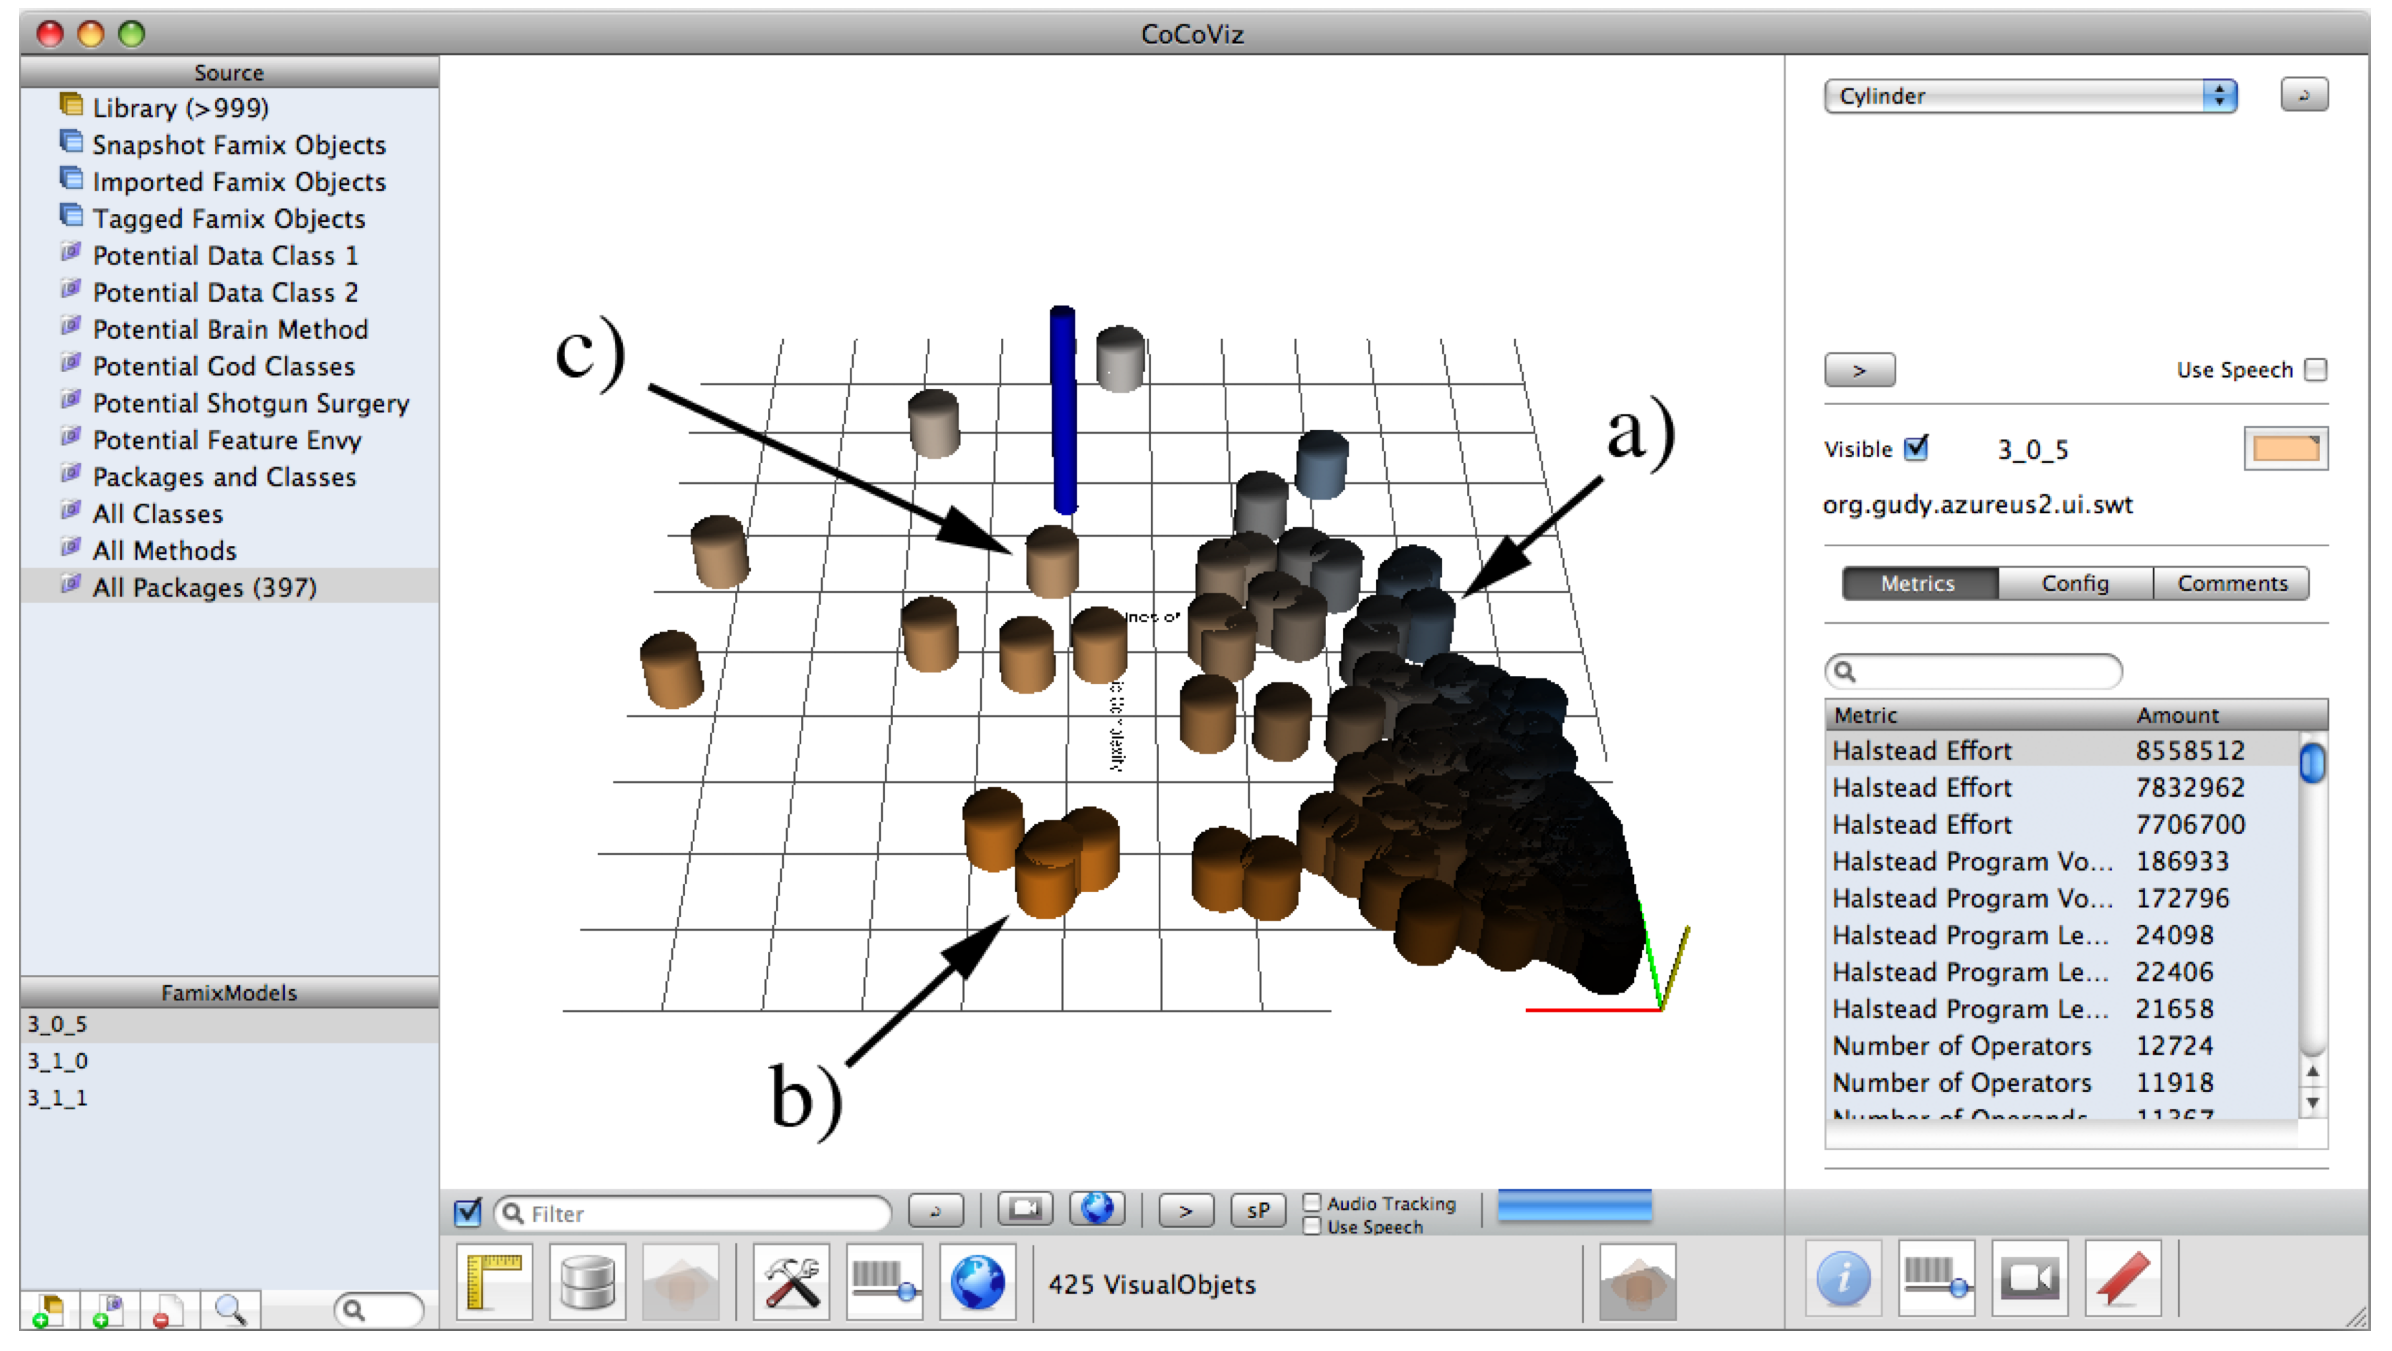
\includegraphics[width=0.9\linewidth]{CocoViz.png} 
  \caption{CocoViz}
\end{figure}



% Orchestrating change: An artistic representation of software evolution https://ieeexplore.ieee.org/document/6747192 
McIntosh et al. \cite{McIntosh2014} explored the use of a parameter-based sonification, to produce a musical interpretation of the evolution of a software system.
They technique mapped musical rests to inactive period of development and consonance and dissonance to interersting phenomena (like co-changing of components).

% Software Musification https://ieeexplore.ieee.org/document/8107958
Mancino and Scanniello \cite{Mancino2017} presented an approach to transform source code metrics in a musical score that can be both visualized and played. 
